\documentclass[]{aiaa-tc} % insert '[draft]' option to show overfull boxes

 \title{A Graph Theory Based Approach to MDAO Problem Formulation}
        
\author{
  David Pate, %
     \thanks{Georgia Tech}
  Dr. Brian German 
     \thanks{Georgia Tech...}
  Justin Gray,%
     \thanks{Aerospace Engineer, MDAO Branch, Mail Stop 5-11, AIAA Member}   
 }
 
%\usepackage{setspace}
%\doublespace

\usepackage{graphicx}
\usepackage{wrapfig}
\usepackage{caption} 
\usepackage{amsmath}
\usepackage{amssymb}
\usepackage{amsfonts}
\usepackage{lscape}
\usepackage{hyperref}
\usepackage{appendix}
\usepackage[section]{placeins}
\usepackage[retainorgcmds]{IEEEtrantools}
\usepackage{subfigure}
\usepackage{comment}
\usepackage{booktabs}

\captionsetup[figure]{margin=5pt,font=small,labelfont=bf,textfont=bf,justification=justified,}
%\captionsetup[wrapfigure]{margin=5pt,font=small,labelfont=bf,justification=justified,singlelinecheck=off}
\captionsetup[table]{margin=5pt,font=small,labelfont=bf,textfont=bf,justification=justified,position=top}

\bibliographystyle{aiaa}

\usepackage{lettrine}
\usepackage{verbatim}

\newcommand{\txt}{\textrm}

%\usepackage{hyperref} %allows for the creation of actual text links
\begin{document}

\maketitle
 
\begin{abstract}
   blah blah blah
\end{abstract}

\section*{Nomenclature}

\begin{tabular}{l l} 
    AAO      & All-At- \\
    MDAO     & Multidisciplinary Design Analysis and Optimization \\
    FPF      & Fundamental Problem Formulation \\
\end{tabular}


\section{Introduction}
    \label{s:intro}
    The number of analysis tools required in multidisciplinary design optimization (MDO) studies is growing
    in parallel with the increasing scope of typical problems. An example can
    be observed in the historical evolution of the disciplines involved in MDO problems in aircraft design.
    Multidisciplinary optimization emerged as a separate field from structural optimization through the
    need to introduce formal techniques for managing the coupling of aerodynamic loads and structural
    deformations, through the linking of aerodynamic vortex lattice or panel methods with structural finite
    element models \cite{Cramer1994}. Subsequently, flight performance and life cycle economics tools were integrated
    into MDO analysis workflows for conceptual and preliminary design studies \cite{Sobieski1998}. Currently, MDO
    problems for aircraft design also often include tools for aircraft noise and emissions. In sum, it is now
    commonplace for 5--10 analysis tools to be employed for typical aircraft design optimization studies.
    
    The number of analysis tools is expected to grow in the future as the scope of MDO problems continues
    to evolve, and as computing is increasingly commoditized. This expansion of scope will be driven, in
    part, by consideration of additional disciplines. Current trends on the horizon for aircraft MDO studies
    include incorporation of manufacturing analyses \cite{deWeck2007}, subsystem performance \cite{Dean2009,Gavel2006}, and models of emissions, noise, or economics \cite{Antoine2004,Rallabhandi2007,Kirby2008}.

    Multidisciplinary Design Analysis and Optimization (MDAO)
    frameworks such as iSight\textsuperscript{\textregistered},\\ ModelCenter\textsuperscript{\textregistered}, ModeFrontier\textsuperscript{\textregistered}, and OpenMDAO\cite{Gray2012} have enabled a new level of analysis tool integration 
    and have paved the way for models with more analyses and increasing numbers of interdisciplinary couplings. This 
    new capability for tool integration has created a new challenge. Even models with tens of analyses could include hundreds or thousands
    of variables that are interdependent and must be linked in the framework.
     
    A common situation is that different analyses provide differing predictions for the 
    same physical quantity, often in different data formats, and these conflicts need to be resolved. 
    These occurrences are particularly acute in situations in which analysis tools have differing fidelities. For
    example, an abstracted aerodynamic analysis such as an empirical drag buildup model may return only
    integrated drag, whereas a CFD tool may return pressure and shear stress distributions across the entire
    surface grid. If an analysis downstream of the aerodynamics tool needs only integrated drag as an input,
    then the designer has a free choice of which of the two possible aerodynamics analysis tools to select to
    provide the drag estimate (presuming that drag can be computed from surface distributions by a simple
    integration algorithm). On the other hand, if a downstream analysis needs a pressure distribution in
    order to compute pitching moment, for example, then any feasible MDO problem formulation must
    include CFD or similar analysis in the data flow, regardless of whether the empirical drag buildup model
    is also included.

    With the added complexity from larger models, it is plausible that the task of combining all the analyses into a 
    consistent system model capable of solving a relevant engineering design 
    problem could approach the cost and time requirements of creating any of the discipline 
    analyses themselves. For these large scale MDO problems, the couplings between the 
    analyses begin to dominate the effort required in setting up the model. It is this problem of 
    determining sets of analysis tools and their inter-connectivities to form realistic
    multidisciplinary problems that is the subject of this paper. We are motivated by the following notional
    but realistic problem of organizing an MDO study for a complex system:

    \begin{quote}
    A new system is being designed for which there is little or no historical precedent. The system
    is complex, as measured by the number of coupled disciplines and/or components involved in the
    analysis. A general optimization problem statement has been formulated based on system-level objectives and constraints; however, it is unclear which engineering analysis tools should
    be interconnected in order to solve the optimization problem. A team of disciplinary and/or component design engineers has been formed in which each engineer has expertise in a
    particular analysis tool or component model. The engineers meet to discuss the approach to
    interconnecting their tools to achieve the required system-level MDO model.
    \end{quote}

    Our goal is to develop formalism for expressing analysis interconnectivity and for determining feasible
    analysis tool sets to assist an engineering team conducting this task. Because the problem deals with
    interconnectivity, we base our approach on the representations and techniques of graph theory.
    The approach begins by constructing the \emph{maximal connectivity graph (MCG)} describing all possible
    interconnections between the analysis tools proposed by the engineers. Graph operations are then
    conducted to reduce the MCG to a \emph{fundamental problem graph (FPG)} that describes a set of analysis
    tools that collectively specify a system-level design problem. The concept of the FPG and the identification of feasible FPGs from an MCG are the main contributions of the paper.

    The information in an FPG represents the engineering design problem that needs to be solved, but the FPG does not 
    itself provide sufficient information to run a design optimization. In particular, it does not provide information 
    about \textit{how} to solve the problem. Even after the problem is defined, an integration platform or framework needs 
    to be selected and appropriate optimization methods identified. This last step essentially 
    involves converting the FPG into a usable model. We briefly consider methods to further 
    manipulate the FPG into a \emph{problem solution graph (PSG)} which could be useful in this 
    task, but the PSG is not the primary focus of this paper. Rather, the work is primarily concerned with applying graph 
    theory to the creation of an FPG and the benefits to the design process obtained by doing so. 
    
    The paper is organized as follows. First, we describe the differences between a fundamental problem
    formulation, which is based only on the system-level optimization problem statement that the
    engineers desire to solve and on the available analysis tools, and a specific problem formulation, which
    additionally presumes a specific MDO solution approach to the problem. Next, we survey the literature related to
    graph theoretic and formal language approaches to multidisciplinary design problem formulation. 
    We then discuss our graph syntax and representation of MDO problems and describe the procedures for 
    determining the MCG and FPG. Finally, we present an example problem based on an MDO analysis of a 
    commercial aircraft.

\section{Background}
\subsection{Specific vs Fundamental Problem Formulation }
	\label{s:specific vs fundamental}
    The Fundamental Problem Formulation (FPF) is our terminology for a statement of the overall system-level optimization problem that contains only  information about analysis tools, design variables, objectives, and constraints without reference to a solution approach. 
In particular, the FPF does not depend on the choice of solution-specific elements such as the MDAO framework, optimization algorithm, iterative solver, or execution sequence. 
This description represents  the problem from the point of view of an engineer specifying the design problem that he/she desires to solve without specifying how the problem should be solved. 
The lack of solution information in the FPF contrasts with optimization problem statements that are written with reference to a specific solution strategy or with implication of a specific execution sequence. 
For example, consider the Sellar test problem \cite{AIAA:sellar} with an FPF given as follows:
    \begin{align}
        \txt{given} & \ \ y_1 = D_1(x_1,y_2,z_1,z_2) \notag
        \\      & \ \ y_2 = D_2(y_1,z_1,z_2) \notag
        \\\txt{min.} &\ \ F(x_1,y_1,y_2,z_2) \notag
        \\\txt{w.r.t.} & \ \ x_1,y_1,y_2,z_1,z_2 \notag
        \\\txt{s.t.} & \ \ G_1(y_1) \geq 0 \notag
        \\     & \ \ G_2(y_2) \geq 0
        \label{eqn:simple_fpf}
    \end{align}
    In Eq.~\ref{eqn:simple_fpf}, $y_1$ is an output of $D_1$ as well as an input 
    to $D_2$. Similarly, $y_2$ is an output of $D_2$ as well as an input 
    to $D_1$. This structure implies that $D_1$ and $D_2$ are coupled together by means 
    of their mutual dependence. However, no information is given as to whether
    $D_1$ or $D_2$ should be executed before the other. Given Eq.~\ref{eqn:simple_fpf}, 
    it would be equally valid to execute $D_1$ first, $D_2$ first, or both simultaneously. 
An MDAO root finding method or compatibility constraint formulation could be implemented to achieve consistency between $D_1$ and $D_2$.
    
    The Sellar problem is simple, with only a single coupling interaction 
    between the two disciplines and a very limited set of variables. 
 However, for larger and more complex problems, 
    it is much more difficult to identify the fundamental problem formulation. Interdisciplinary 
    couplings are not always apparent and the set of analysis tools and variables are 
    much larger. 

An example of a more specific problem statement for the Sellar problem is presented in Eq. 2.  
In this formulation, the implication is that  $D_1$ must be run 
    first. A new variable, $\hat{y_2}$, is introduced to break the direct dependence of
    $D_1$ on $D_2$, and a new coupling constraint, $H$, is added to enforce 
    consistency. Equation \ref{eqn:simple} is 
    an equally valid expression of the Sellar problem that could be 
    generated  based on a preferred solution approach.
    \begin{align}
        \txt{given} & \ \ y_1 = D_1(x_1,\hat{y_2},z_1,z_2) \notag
        \\      & \ \ y_2 = D_2(y_1,z_1,z_2) \notag
        \\\txt{min.} &\ \ F(x_1,y_1,y_2,z_2) \notag
        \\\txt{w.r.t.} & \ \ x_1,y_1,\hat{y_2},z_1,z_2 \notag
        \\\txt{s.t.} & \ \ H(y_2,\hat{y_2}) = 0 \notag 
        \\     & \ \ G_1(y_1) \geq 0 \notag
        \\     & \ \ G_2(y_2) \geq 0
        \label{eqn:simple}
    \end{align}
\subsection{Background in Graph-Based Descriptions of MDAO Problems}
	\label{s:existing syntax}
    As indicated in the examples in Sec.~\ref{s:specific vs fundamental}, the mathematical 
    language for specifying optimization problem formulations is very general and can be used both for 
    fundamental and specific problem formulations. Tedford and Martins used this syntax to specify the 
    FPF for a set of test problems and also to describe specific formulations for solving them with a 
    number of optimization architectures \cite{Tedford2009}. By solving different specific problem statements corresponding to the same FPF, they were able to  benchmark the performance of different optimization architectures against a fixed set of 
    problems. Gray et al. also benchmarked the performance of a set of MDAO architectures  with a similar approach \cite{Gray2013}. 
    This work examined a larger set of architectures and proposed the use of OpenMDAO as a platform to build a larger community-developed set of test problems and architectures. Both of these benchmarking efforts 
    demonstrate how multiple specific problem formulations can relate to a common FPF and indicate the 
    value of a common problem description. The challenge with this 
    traditional syntax is that it is not easily manipulated or analyzed with automatic procedures to explore alternate problem formulations. 

    A number of graph-based methods have been used successfully to translate the 
    mathematical syntax into a more useful computational form. 
    Steward's Design Structure Matrix (DSM) is a square adjacency matrix which captures the relationship between analysis tools \cite{Steward1981}.
    Off-diagonal elements of the matrix indicate coupling. Since a DSM describes a square adjacency matrix, 
    it can be represented as an equivalent directed graph in which nodes represent analysis tools and 
    edges represent information dependence between those tools. The ordering of elements in a DSM can be used to indicate 
    execution order.  For more complex problems, choosing the proper order to run analysis tools is a challenging task. 
    Rogers et al.~developed DeMAID to manipulate a DSM to find an ordering for analysis tools that 
    reduces the cost of solving highly coupled systems \cite{rogers1996,rogers1996demaid}. This re-ordering is done through 
    operations on the DSM matrix and yields multiple specific problem 
    formulations which all solve the same FPF. 
    
    A DSM itself is insufficient to describe complete optimization problem formulations because it 
    captures only information about data dependency between analyses; objective and 
    constraint information is missing from the DSM description of the problem. 
    An alternative matrix-based syntax, called a Functional Dependency Table (FDT), was proposed by Wagner and Papalambros \cite{Wagner1993}. 
    The FDT represents the relationship between functions, including objectives and constraints, and specific variables that affect 
    them. Similar to DSM, FDT also describes an adjacency matrix of a graph. Unlike the DSM graph, 
    however, the FDT graph is undirected and nodes can represent analysis tools, objectives, 
    or constraints. Edges between nodes represent a dependence on the same 
    variable. Michelena and Papalambros made use of the FDT to solve a graph partitioning problem that yielded 
    more efficient optimization problem decompositions \cite{Michelena1997}. Allison 
    extended this work to incorporate adjacency matrix information with the FDT to 
    account for system coupling in an automated partitioning scheme \cite{Allison2008}. 

    Although FDT succeeds at capturing the 
    information about objectives and constraints, its lack of directed edges 
    implies that it cannot describe the coupled data dependency that a DSM captures. 
    Table \ref{t:FDT_simple}  shows the FDT for the Sellar problem described by Eq.~\ref{eqn:simple_fpf}.
    The FDT indicates that $D_1$ is dependent on $y_2$ and 
    that $D_2$ is dependent on $y_1$, but the coupled dependence cannot be inferred from 
    that information alone. This missing information implies 
    that, although FDT is very useful for partitioning problems, it is not 
    sufficient to completely describe the data flows in a problem formulation. 

\begin{table}[htb!]
  \centering
        \caption{Sellar Problem FDT}
        \begin{tabular}{|c|c|c|c|c|c|c|}
            \hline
                   & $x_1$ & $y_1$ & $y_2$ & $z_1$ & $z_2$ \\ \hline
            $D_1$  & 1     &       & 1     & 1     & 1     \\ \hline
            $D_2$  &       & 1     &       & 1     & 1     \\ \hline
            $F$    & 1     & 1     & 1     &       & 1     \\ \hline
            $G_1$  &       & 1     &       &       &       \\ \hline
            $G_2$  &       &       & 1     &       &       \\
            \hline
        \end{tabular}
 \label{t:FDT_simple}
\end{table}%

    Alexandrov and Lewis introduced a graph based syntax called Reconfigurability in 
    MDO Problem Synthesis (REMS) which incorporates objectives and constraints 
    into a graph, effectively combining FDT and DSM \cite{alexandrov2004}. REMS retains the square adjacency 
    matrix from DSM, but by adding the objectives and constraints, it partially 
    combines a traditional DSM with an FDT. This formulation allows REMS to represent data 
    dependency between multiple analysis tools as well as between analysis tools and
    objective/constraint functions. Additionally, REMS addresses the need to
    transition between multiple solution strategies while maintaining a single consistent  
    graph representation of the fundamental problem formulation. However, REMS does not provide 
    a mechanism for inclusion of solvers or optimizers in the graph. This fundamentally limits REMS 
    from describing the specifics of different solution strategies as applied to a specific problem. 

    Lamb and Martins also included objectives and constraint functions as nodes 
    in an Extended DSM (XDSM) in order to capture a more complete description 
    of solution strategies for MDAO problems \cite{Lambe2012}. Unlike REMS, 
    XDSM also includes nodes for solvers and optimizers to enable complete 
    definition of MDAO architectures. Martins uses XDSM to describe thirteen different 
    optimization architectures in a survey paper that provides a novel 
    classification of the different techniques \cite{Lambe2011}. With the 
    additional information included in an XDSM, Lu and Martins applied both 
    ordering and partitioning algorithms to an MDAO test problem termed the 
    Scalable Problem \cite{Lu2012}. 

    \begin{figure}
        \begin{center}
        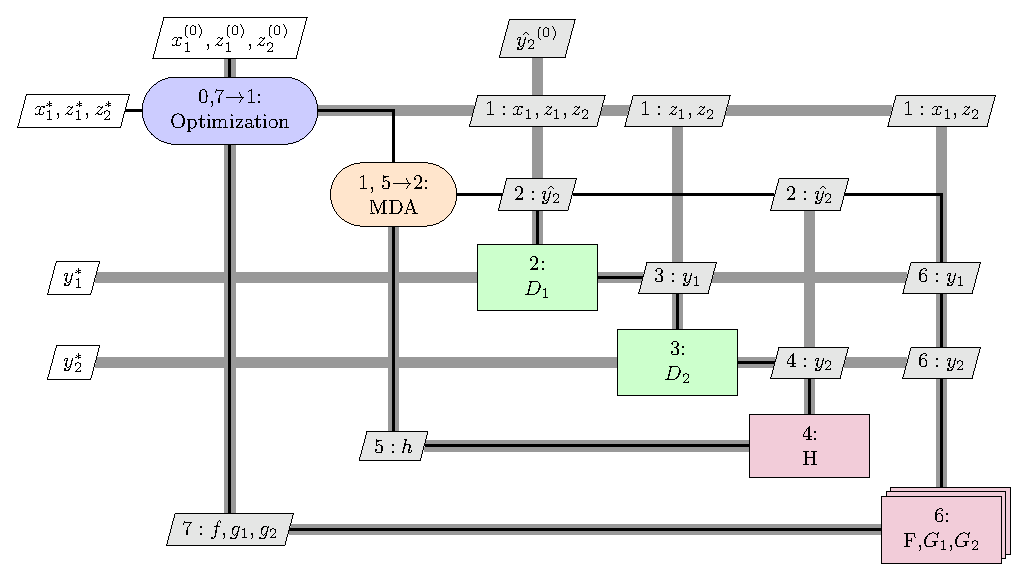
\includegraphics[height=.25\textheight]{XDSM/simple}
        \caption{XDSM for Eq. \ref{eqn:simple}, with a Gauss-Seidel iteration 
          and MDF solution architecture. \label{fig:XDSM_simple}}
        \end{center}
    \end{figure}

    Although XDSM captures many of the functional aspects of FDT, it 
    requires the use of solver and optimizer blocks to represent 
    the relationship between design variables and objectives/constraints. 
    By introducing solver or optimizer blocks, XDSM automatically implies a solution strategy. 
    The XDSM for Eq. \ref{eqn:simple} is given in Figure \ref{fig:XDSM_simple}. 
    This diagram is shown with an assumed Gauss-Seidel iteration scheme and an MDF solution architecture. 

    In this paper, we propose a new graph syntax that combines certain features of REMS and XDSM. 
    Despite sharing some features with both of these other graph based approaches, the syntax
    proposed here has a fundamentally different goal which is complementary to both of them. 
    REMS and XDSM provide excellent human readable formats for an MDAO problem description, whereas the  
    syntax described in this paper is designed to provide an effective machine readable format for MDAO problem definition. 
    In the interest of simplifying algorithmic operations on the graphs, the specified 
    format is both more verbose and less visually informative. The benefit is a consistent 
    and easily utilized graph from a algorithmic perspective. 

\subsection{Requirements for a New Graph Syntax}
  \label{s:requirements}
  The goal of the graph-based syntax presented here is to enable the general 
  structure of an MDAO problem to be described independently of any solution information, 
  while still being able to accommodate the more specific case when a solution 
  strategy is applied. In order to achieve this goal, 
  the graph syntax needs to accommodate a number of MDAO problem constructs: 
  \begin{itemize}
    \item Analysis tools and their interconnections
    \item Design variables, objectives, and constraints
    \item Coupling between analyses
    \item Multi-fidelity analyses
  \end{itemize}

  The syntax is intended to represent three phases of the design problem 
  formulation process. In the initial problem definition phase, the specific 
  analysis tools and design goals are identified. Next, a single problem 
  formulation is identified that specifies design variables, constraints, 
  objectives, analysis tools, and all other elements required to represent 
  the overall MDAO problem. Lastly, a specific procedure for solving the problem 
  is selected, e.g. an MDAO optimization architecture. Using 
  the proposed graph syntax, the outcome of these phases can be represented with the following graphs:
  \begin{itemize}
    \item Maximal Connectivity Graph (MCG)
    \item Fundamental Problem Graph (FPG)
    \item Problem Solution Graph (PSG)
  \end{itemize}

  The \emph{maximal connectivity graph} represents the first phase of the problem 
  formulation with all analysis tools being considered and all possible connections 
  between them also present. The second phase of problem formulation results in the \emph{fundamental problem graph}, 
  which comprises only the analysis tools, objectives, constraints, and variables to solve the problem. 
  The final phase results in a \emph{problem solution graph} which includes additional 
  edges and nodes to represent the solution strategy being employed to solve the 
  problem.

  Comparisons of the number and size of each of these graphs are depicted in Figs.~\ref{f:tree} and \ref{f:hourglass}. 
  The tree diagram illustrates that it is generally possible to obtain 
  multiple FPGs from a single maximal connectivity graph. The multiple FPGs may correspond to 
  different down-selections of analysis tools, different connections between the tools, 
  or both. Each down-selection reduces the number of possible FPGs that could be reached 
  until only one remains. For a given FPG, however, different PSGs may be obtained by implementing 
  different solution strategies. Considering the size of a graph to be the sum of all of its
  edges and nodes, the hourglass shape in Fig. \ref{f:hourglass} qualitatively illustrates how
  the FPG is obtained from the MCG by \emph{removing} nodes and edges, 
  and the PSG is obtained from the FPG by \emph{adding} nodes and edges.
These additions correspond to optimizers, solvers, and compatibility constraints required in particular MDAO solution architectures.
\begin{figure}[htb!]
    \centering
    \subfigure[Number of possible graphs]{
    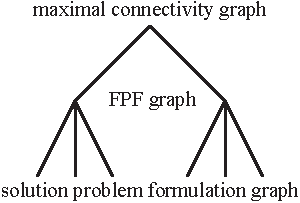
\includegraphics[width=1.75in]{images/tree}
    \label{f:tree}
    }
    \subfigure[Graph size]{
    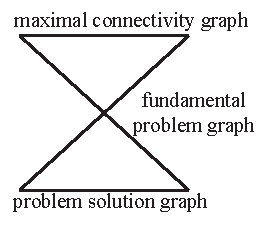
\includegraphics[width=1.75in]{images/hourglass}
    \label{f:hourglass}
    }
  \caption{The relationship between the MCG, FPG, and PSG.}
  \end{figure}

\subsection{Potential Applications}

The syntax proposed here for defining graphs is partially motivated by the unique needs
in formulating very large problems that have thousands of design variables. Such problems are 
large enough that many traditional design methods stumble simply because one person cannot maintain a complete view of the problem. Hence, as problems 
grow, software tools become needed to manage the complexity of the problem itself. 

Even for small problems, algorithmic exploration of problem structure can yield deeper understanding 
of problems and more effective solution methods, as demonstrated by the work by Michelena and Papalambros \cite{Michelena1997} and Allison \cite{Allison2008} in applying FDT to study problem partitioning. The syntax and rule set described 
in this paper
provide a foundation for the development of new algorithms for analyzing and modifying 
problem structure. This foundation is intended to facilitate a standard view of 
problem definition and automatic methods for investigating different  problem formulations within MDAO frameworks. 


\section{Graph--based Problem Formulation Syntax}
A problem formulation will be represented by nodes and edges which will be assigned certain properties and rules. There are many MDAO problem formulation concepts that we wish to represent. An analysis code should be represented by a distinct structure to distinguish between the input, output, and function evaluation, processes. The variables passed between analysis codes should be represented separately to provide insight and control over the dataflow. For example, it is important to distinguish between the case where two analysis codes are supplying the same variable to a third code, or the case where the two analysis codes are providing different variables to the third code. 
Local inputs, local outputs, and design variables(??) should be distinguished from global inputs, which are input that are used by multiple analysis codes.
Objectives and constaints should be represented as separate from local variables because they must be provided in order for the problem formulation to be valid. The coupling between sets of analysis codes is important to capture, and multi--fidelity analysis should also be allowed.

\subsection{Graph Theory Basics}
We begin by discussing the general syntax of graph theory and then expand upon this syntax to represent the data flow of an MDAO problem. The present notation is adapted from Diestel \cite{Diestel2010}.
A \emph{graph} is a pair $G = (V,E)$ of sets such that $E \subseteq V \times V$, which means that the elements of $E$ are 2--element subsets of $V$. The set $V$ contains the \emph{vertices} or \emph{nodes} and the set $E$ contains the \emph{edges}.
For a \emph{directed graph*} we construct $E$ as a set of ordered pairs instead of a set of sets. Each ordered pair represents an edge starting at the node indicated by the first entry and directed to the node indicated by the second entry. Edge $e$ = $(x,y)$ may be referred to simply as $xy$ and we say $y = E(x)$. 
\begin{figure}[htb!]
	\begin{center}
	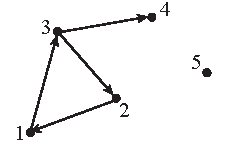
\includegraphics[width=1.5in]{images/example_directed_graph}
	\end{center}
	\vspace{-20pt}
\caption{Example directed graph.}
\label{f:example directed graph}
\end{figure}
As an example, for the directed graph shown in Fig.~\ref{f:example directed graph} we have
\begin{IEEEeqnarray*}{rCl}
V & = & \{1,2,3,4,5\}, \\
E & = & \big\{(1,2),(3,2),(1,3),(3,4)\big\}.
\end{IEEEeqnarray*}

% \subsection{Problem Formulation Concepts to Represent}
% The MDAO problem formulation concepts we wish to represent are:
% \begin{description}
% \item[global input] A global input is a variable that is taken as given and is used by multiple analyses.
% \item[design variable]
% \item[function call] A function call requires a set of inputs to be fulfilled and has certain properties, such as run time, which are independent of the number of outputs actually being used.
% \item[passing of distinct variables] Instead of connecting analyses, the individual variables as are connected
% \item[objective \& constraint] These are variables that must be produced by the problem formulation for it to be valid
% \item[collision] A collision occurs when an input has multiple sources
% \item[hole] A hole occurs when an input has no sources
% \item[coupling] Couple is the mutual dependence between a set of analysis
% \item[multi--fidelity] It may be desirable for the same variable to be calculated by separate analyses and to use both results.
% \end{description}

\subsection{Graph Theory Representation of a Problem Formulation}
In order to represent the listed problem formulation concepts with a graph, we assign properties and rules to nodes and edges.
The first property assigned to nodes and edges is the \emph{type}. \\
The possible node types are:
\begin{description}
\item[variable node] The variable node represents passing of data.
\item[model node] The model node represents the handling of data.
\end{description}
The possible edge types are:
\begin{description}
\item[fixed edge] A fixed edge may not be removed.
\item[free edge] A free edge may be removed.
\end{description}
Model nodes must be used with the following rules:
\begin{itemize}
\item A model node can only have one edge directed to or from another model node.
\item A model node can only have fixed edges directed in or out.
\item A model node must have at least one edge directed in and at least one edge directed out.
\end{itemize}
The MDO problem formulation concepts represented by nodes are given in Table \ref{t:node representation}, and the concepts represented by nodes are given in Table \ref{t:edge representation}.
% \begin{itemize}
% \item An objective or constraint is indicated by a variable node with no outgoing edges and with the incoming edges being directed from only other variable nodes.
% \item A global input is a variable node with no edges directed in and with at least two edges directed out to different variable nodes.
% \item A design variable is represented by a variable node with no edges directed in and on fixed edge directed out.
% \end{itemize}
\begin{table}[h!]
 \begin{center}
  \caption{Problem formulation concept represented by a node}
  \label{t:node representation}
  \begin{tabular}{ccc} \hline 
edges directed in & edges directed out & node representation \\ \hline
only free edges & none & objective or constraint\\
none & at least two free edges & global input \\
none & one fixed edge & design variable \\ \hline
  \end{tabular}
 \end{center}
 \vspace{-15pt}
\end{table}
\begin{table}[h!]
 \begin{center}
  \caption{Problem formulation concept represented by an edge}
  \label{t:edge representation}
  \begin{tabular}{ccc} \hline 
from node & to node & edge representation \\ \hline
variable & variable & connection/passing of a variable\\
variable & model & local input \\
model & variable & local output \\
model & model & function call \\ \hline
  \end{tabular}
 \end{center}
 \vspace{-15pt}
\end{table}

Finally, an analysis code is represented by an \emph{analysis block}, which is a collection of model nodes, variable nodes, and fixed edges with a specific structure. This structure is derived from the need to represent each input and output individually while representing the actual analysis with a single node or edge. The variable nodes each represent a single input or output of the analysis block. Each of these nodes is connected to a single model node via a fixed edge, which represents the gathering of the inputs to begin the analysis or the disseminating of outputs after the analysis. Finally, free edges are used to connect the variable nodes of the analysis block to other variables nodes outside of the analysis block. In this way, the analysis block graph is a fundamental building block of the MDAO problem data flow.
\begin{figure}[htb!]
	\begin{center}
	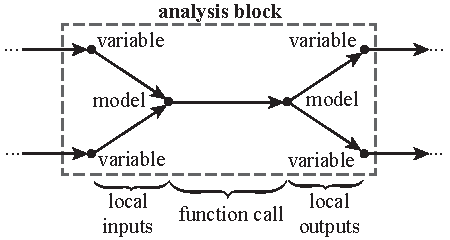
\includegraphics[width=4in]{images/analysis_block}
	\end{center}
	\vspace{-10pt}
\caption{Example analysis block. The each node type and edge type is labeled in italics and annotated parenthetically.}
\label{f:analysis block}
\end{figure}
%`Connection' edges connect the local outputs from one analysis block to input nodes.

\section{Graph--based Representation of the Fundamental Problem Formulation}
Next we provide the meaningful graphs that can be created from the suggested syntax. The first graph is the \emph{maximal connectivity graph} which represents the full potential of all the analysis codes being considered, i.e. each analysis code is represented by an analysis block, and each potential connections between variables is represented by a free edge. The second graph that may be represented is \emph{fundamental problem formulation graph}, which is the graph with the fewest number of edges and nodes needed to provide a valid problem formulation, as disscussed subsequently. Finally, a \emph{solution problem formulation} may be represented by including additional edges and node times to represent the optimization architecture, though this is beyond the scope of this paper. 

The relationship between these three graphs is depicted in Figs.~\ref{f:tree} and \ref{f:hourglass}. The tree diagram demonstrates the fact that it is generally possible to obtain multiple FPFs from a single maximal connectivity graph. This  may correspond to different down--selections of analysis codes, different connections between them, or both. Then, for each FPF, different SPFs may be obtained by implementing different optimization architectures. The hourglass shape indicates that the FPF graph is the smallest graph that may represent a specific problem formulation. The FPF is obtained from the MCG by removing nodes and edges, and the SPF is obtained from the FPF by adding nodes and edges.
\begin{figure}[htb!]
	\centering
	\subfigure[number of possible graphs]{
	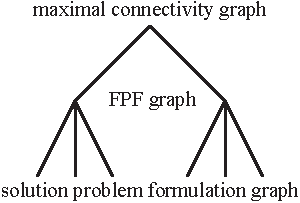
\includegraphics[width=2.0in]{images/tree}
	\label{f:tree}
	}
	\subfigure[graph size]{
	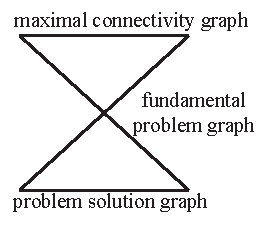
\includegraphics[width=2.0in]{images/hourglass}
	\label{f:hourglass}
	}
\caption{The relationship between the MCG, FPF, and SPF.}
\end{figure}

In this section we introduce the remaining necessary notion and give graph--theory based definitions of the MCG and FPF, and then process to demonstrate how the FPF is obtained from the MCG.

\subsection{Additional Notation}
For node $v \in V$ the edges directed out are given by $E(v)$ and the edges directed into $v$ are given by $E^{-1}(v)$; $E(E(v))$ is denoted as $E^2(v)$, and likewise for additional levels. 
The \emph{indegree} of a node is the number of edges directed in and is denoted as $\txt{deg}^-(v)$, and the \emph{outdegree} is the number of edges directed out and it is denoted as $\txt{deg}^+(v)$.
We also define the \emph{upper indegree limit} 
\begin{equation}
\txt{deg}_u^-(v):V \to \mathbb{N}
\end{equation} 
and the \emph{lower indegree limit}
\begin{equation}
\txt{deg}_l^-(v):V \to \mathbb{N}.
\end{equation}
These user-specified limits set the number of edges that may be directed into a node for a problem formulation to be valid. For example, a variable node $v$ will have $\txt{deg}_u^-(v) = \txt{deg}_l^-(v) = 1$, unless it is a multi--fidelity variable, in which case the user may specify some upper limit higher than one.

To keep track of which nodes and edges are which type, let $T_\txt{node}$ and $T_\txt{edge}$ be sets containing the possible node types and edge types, respectively, and then define mappings $t_\txt{node}:V \to T_\txt{node}$ and $t_\txt{edge}:E \to T_\txt{edge}$ to assign a type to each node and edge.
Then, for example, for a variable node $v$ we have $t_\txt{node}(v) = \txt{`variable'}$.


 % A \emph{path} is a nonempty graph $P = (V,E)$ with $V = \{x_0,x_1,\ldots,x_k\}$ and $E = \{x_0x_1,x_1x_2,\ldots,x_{k-1}x_k\}$, where $x_i$ are all distinct. A graph $G$ is \emph{connected} if any two of its vertices are linked by a path in $G$. A \emph{tree} is a connected and acyclic graph.
%%% this needs to be changed to fit the definition using a directed graph


\subsection{Maximal Connectivity Graph}
To construct the maximal connectivity graph, we assume that a set of codes, global inputs, and objectives and constraints (collectively called global outputs). The codes are represented by analysis blocks $A_i=(V_{A_i},E_{A_i}), \ i=1,\ldots,m$, the global inputs are represented a set of variable nodes $I$, and the global outputs are represented by a set of variable nodes $O$. We assume that $O$, $I$, and $A_i$ are given, and that any potential connection between variables is given in the form of the free edges in the set $C_M$. 
Then we may construct the maximal connectivity graph $M=(V_M,E_M)$ as
\begin{IEEEeqnarray*}{rCl}
V_M & = & I \cup O \cup \left( \bigcup_{i = 1}^m V_{A_i} \right), \\
E_M & = & C_M \cup \left( \bigcup_{i=1}^m E_{A_i} \right),
\end{IEEEeqnarray*}
The MCG $M$ is uniquely determined by the given set of analysis blocks, the required outputs, and the given global inputs. In the cases where the set of global inputs $I$ is not known a priori, the process of obtaining the FPF will reveal the required inputs, as discussed subsequently.

\subsection{Fundamental Problem Formulation Graph}
We now define the fundamental problem formulation graph, $F=(V_F,E_F)$, as a directed graph meeting the following conditions
\begin{enumerate}
\item[(1)] $\displaystyle{V_F = I_F \cup O \cup \left( \bigcup_{i \in \mathcal A} V_{A_i} \right),\ I_F \subset I}$
\item[(2)] $\displaystyle{E_F = C_F \cup \left( \bigcup_{i \in \mathcal A} E_{A_i} \right)}$
\item[(3)] $\displaystyle{\forall v \in V_F \txt{ with } t_\txt{node}(v) = \txt{`variable,'}\quad \txt{deg}_l^-(v) < \txt{deg}^-(v) \leq \txt{deg}_u^-(v)}$
\end{enumerate}
The set $\mathcal A$ is an index set containing the indices of the analysis blocks in $F$; for the case where all of the analysis blocks are used, we would have $\mathcal A = \{1,2,\ldots,m\}$. The first requirement for $F$ is that $V_F$ be composed of all of the global outputs (the required objectives and constraints), the nodes from each analysis block in $F$, and any global input nodes that are needed, $I_F$. The second requirement suggests that the edges in $F$ comprise the edges for each analysis block and the edges between them, the global inputs, and the global outputs. The final requirement is specific to the number of edges directed into a variable. If there are no edges directed inward, the node is called a \emph{hole}, and if more connections are directed in than are allowed, the node is called a \emph{collision}; a hole is allowed if $\txt{deg}_l^-(v)=0$. The final requirement is therefore a requirement on $C_F$.

\subsection{Obtaining the Fundamental Problem Formulation Graph}
In general, there may be multiple different graphs that satisfy the FPF conditions, though there may be none at all. Here, we describe a process for obtaining an FPF by starting with the MCG and disconnecting free edges until the FPF conditions are met. Then the problem is reduced to deciding which free edges to remove.

%Then, mathematically, the FPF starts with $\mathcal A_1 = \{1,\ldots,m\}$, $I_{F,1} = I$, and $C_{F,1} = C_M$.
Then, mathematically, the FPF starts with $C_{F,0} = C_M$.
First address the nodes where $\txt{deg}^-(v) < \txt{deg}_l^-(v)$ then the ones where $\txt{deg}^-(v) > \txt{deg}_u^-(v)$

\begin{enumerate}
\item The first step is to detect holes and disconnect the free edges following them. These free edges are removed because they represent variables which cannot be determined because the analysis function does not have adequate inputs. The set of variable nodes which are holes is created as
\begin{equation}
H = \{v \in V | \txt{deg}^-(v) < \txt{deg}_l^-(v) \}
\end{equation}
Then the updated set of edges is
\begin{equation}
C_{F,1} = C_{F,0} \setminus \{\ e \in E, \ e=xy | x=E^3(v) \txt{ for } v \in H\}
\end{equation}
%deg-v is now recaculated for the new C. 
This step is demonstrated by Fig.~\ref{f:holes}.
\item (())
\end{enumerate}
\begin{figure}[htb!]
	\begin{center}
	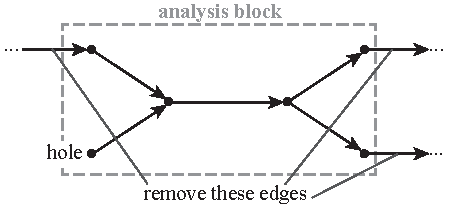
\includegraphics[width=3in]{images/analysis_block_hole}
	\end{center}
	\vspace{-20pt}
\caption{Example variable node indicating a hole.}
\label{f:holes}
\end{figure}


%\begin{enumerate}
%\item The first step is to detect holes and remove the corresponding analysis blocks, which could not be used because the required inputs are not supplied. Any analysis blocks with holes may be stored in an index set $\mathcal H$ as
%\begin{equation}
%\forall i \in \mathcal A_1,\txt{ and }\forall v \in V_{A_i},\txt{ if deg}^-(v)=0 \txt{ then } i \in \mathcal H.
%\end{equation}
%Then an updated index set $\mathcal A_2$ is created using set difference notation as
%\begin{equation}
%\mathcal A_2 = \mathcal A_1 \setminus \mathcal H
%\end{equation}The connection edges directed from the removed analysis blocks are removed as
%\begin{equation}
%H = \{c \in C_{F,1} |c = (e^{-1}(v),v), \txt{ where } v \in V_{A_i} \txt{ for some } i \in \mathcal H\},
%\end{equation}
%\begin{equation}
%C_{F,2} = C_{F,1} \setminus H
%\end{equation}
%Finally, the FPF is updated as
%\begin{equation}
%V_{F,2} = I_{F,2} \cup O \cup \left( \bigcup_{i \in \mathcal A_2} V_{A_i} \right),
%\end{equation}
%\begin{equation}
%E_{F,2} = C_{F,2} \cup \left( \bigcup_{i \in \mathcal A_2} E_{A_i} \right)
%\end{equation}
%This process may require multiple iterations because removing an analysis block may create holes upstream. It is assumed that the process as been repeated sufficiently such that $\mathcal A_2$ does not have any holes.
%
%\item The next step is to resolve conflicts. The set $C$ of input nodes containing conflicts is
%\begin{equation}
%C = \{v \in V_{F,2} | t_\txt{node}(v) = \txt{`input'} \txt{ and } \txt{deg}^-(v) > d(v)\}
%\end{equation}
%%\begin{equation}
%%for v \in c let 
%%\end{equation}
%\end{enumerate}

%\subsection{Classification of the FPF}

%A collision represents a choice.
%Delete edges and analysis blocks so that there are no nodes or collisions.





% \begin{figure}[htb!]
	% \begin{center}
	% 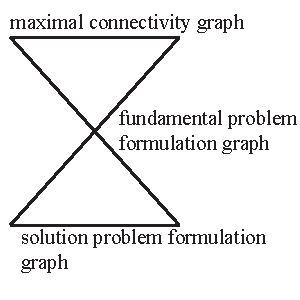
\includegraphics[width=2in]{images/hour_glass}
	% \end{center}
	% \vspace{-20pt}
% \caption{(()).}
% \label{f:our glass}
% \end{figure}
% \subsection{old}
	% For a large scale problem with many analyses, obtaining the FPF is likely to be a challenge. In general, a set of analysis codes will be given and the desired outputs will be specified as
	    % \begin{align}
            % given & \ \ A: \lbrace x_i \lvert i \in A_\textrm{input} \rbrace \rightarrow \lbrace x_i \lvert i \in A_\textrm{output} \rbrace \notag
            % \\    & \ \ B: \lbrace x_i \lvert i \in B_\textrm{input} \rbrace \rightarrow \lbrace x_i \lvert i \in B_\textrm{output} \rbrace \notag
			% \\    & \ \ \quad \quad \quad \quad \quad \quad  \quad \quad \vdots
            % \\min. &\ \ f(x_i), i \in \mathcal{O} \notag
            % \\w.r.t. & \ \ x_i, i \in \mathcal{I}, \notag
            % \label{eqn:preFPF}
        % \end{align}
	% where $\mathcal{O}$ is the index set of the global outputs and $\mathcal{I}$ is the index set of the global inputs. For this to be an FPF, there must be no \emph{conflicts} or \emph{holes}. A conflict arises when different analyses produce the same output; two analysis codes $A$ and $B$ are in conflict if
		% \begin{equation}
			% A_\textrm{output} \cap B_\textrm{output} \neq \emptyset.
		% \end{equation}
	% A hole arises when a local input to an analysis block is neither a global input nor a local output of any analysis block. If we let $\mathcal{H}$ denote the index set of local inputs which are holes
		% \begin{equation}
			% i \in \bigcup \{A_\textrm{input},B_\textrm{input},\ldots\} \textrm{ and } i \notin \bigcup \{\mathcal{I},A_\textrm{output},B_\textrm{output},\ldots\}  \implies  i \in \mathcal{H}.
		% \end{equation}
	% If the given set of analyses contains any holes, an FPF cannot be obtained. On the contrary, if there are conflicts multiple FPFs may be obtained. This is because every conflict represents a choice of which analysis to use and each choice could (potentially) yeild a different but valid FPF. The following section develops an application of graphy theory to obtain multiple FPFs from a set of analyses and desired outputs.
		
    % \subsection{Formulation Graph Syntax}
    % Rather than start with an adjacency, we chose to work directly with a directed cyclic graph to develop a syntax for the FPF. 
    % The following information must be provided to start:
    % \begin{itemize}
        % \item Analysis blocks: an analysis block represents any calculation, and each comes with
            % \begin{itemize}
                % \item local inputs
                % \item local outputs 
                % \item execution properties: these are the properties associated with running the code, such as run time
            % \end{itemize}
        % \item Global parameters: these may serve as fixed inputs to the local inputs of analysis blocks
        % \item Global outputs: these may represent
            % \begin{itemize}
                % \item objectives
                % \item constraints
                % \item residuals: (not sure)
            % \end{itemize}
    % \end{itemize}

    % The graph representation of a data flow is cast to utilize the extensive library of algorithms in graph theory to analyze a directed weighted graph. 
    % Edge weights are used to represent the metrics associated with a data flow:
    % \begin{itemize}
        % \item Run time: this metric is a property of an analysis block
        % \item Fidelity: this metric is a property of an individual local output
        % \item Expected Convergence
    % \end{itemize}

    % The key assumption is that identical variables are recognized as such. This serves as the basis for creating a data flow by connecting compatible input and output nodes with a directed edge. 
    % To represent the fact that execution of an analysis code does not depend on the number of outputs being used, we have created the following figure (not made yet).
    
    % This information immediately leads to the maximal connectivity graph, which is formed by placing a directed edge from each local output or global parameter to each matching local input or global output. 
    % Whenever multiple edges are connected to a single input, a conflict occurs because only one may be used. Resolving these conflicts is one key challenge in creating a data flow.
%    \begin{itemize}
%        \item Specify analyses
%        \item Connections between analyses 
%            \begin{itemize}
%                \item local variables
%                \item global variables? Use "fake" node that broadcasts out to the rest of the graph? 
%            \end{itemize}
%        \item Cycles indicate coupling
%        \item Cycles for design variables->objectives/constraints
%        \item Objectives/constraints are just outputs? Special nodes? 
%        \item Residuals are just outputs? Special nodes? 
%        \item Parameters are just input nodes that are not design variables (use identifies these)
%        \item FPF no solvers/optimizers anywhere in it
%    \end{itemize}

    \subsection{Solution Graph Syntax}
    What is the difference between a problem formulation and a problem solution method? Convert from a cyclic graph, to an acyclic graph
    \begin{itemize}
        \item Cycles indicate convergence loops or design variable loops
        \item Problem can't be solved until all loops are *removed* by adding solvers/optimizers
        \item *Special* nodes for solvers and optimizers that *break* loops (from an algorithmic point of view)
        \item FPF represents the minimal amount of information necessary to define a problem
        \item Any solution path grows the graph complexity by adding edges and nodes (or possibly have an empty solution graph, which you build up
        as you remove edges from problem formulation graph?)
    \end{itemize}

\section{The MCG and FPG}
    \label{s:building graphs}
We now discuss how the graph-based syntax defined in Secs.~\ref{s:syntax definition} and \ref{s:graph representation}  is used to represent an MDAO problem in its entirety. This discussion is based on the MCG and the FPG.

\subsection{Maximal Connectivity Graph}
    \label{ss:MCG}
For a specified MDAO problem, the maximal connectivity graph represents every analysis tool, objective, constraint, and input being considered, as well as every possible interconnection among them.
The definition of the MCG is given via construction.
    To construct the maximal connectivity graph, we presume that a set of analysis tools, inputs, objectives, and constraints are provided. 
    Each of the $m$ analysis codes correspond to an index $i\in I_A$, $I_A=\{1,2,\ldots,m\}$, and are represented by an analysis block graph $G_{A_i}=(V_{A_i},E_{A_i})$.
    Each of the $n$ expression blocks correspond to an index $i\in I_E$, $I_E=\{1,2,\ldots,n\}$, and is represented by expression block graph $G_{E_i}=(V_{E_i},E_{E_i})$.
    Finally, the inputs are represented as a set of variable nodes $V_\txt{in}$.
    We presume that $V_\txt{in}$, each $G_{A_i}$, and each $G_{E_i}$ are given, and that any potential connection between variables is specified in the form of connection edges in the set $E_{M,\txt{con}}$. One method for defining these connections is to use a consistant variable naming convention.

    We may then construct the maximal connectivity graph $M=(V_M,E_M)$ as
    \begin{IEEEeqnarray*}{rCl}
    V_M & = & V_\txt{in} \cup \left( \bigcup_{i \in I_A} V_{A_i} \right) \cup \left( \bigcup_{i \in I_E} V_{E_i} \right), \\
    E_M & = & E_{M,\txt{con}} \cup \left( \bigcup_{i \in I_A} E_{A_i} \right)  \cup \left( \bigcup_{i \in I_E} E_{E_i} \right).
    \end{IEEEeqnarray*}
    The MCG $M$ is uniquely determined by the given set of analysis blocks, inputs, and expression blocks. 
    In the cases where the set of inputs is not known a priori, the process of obtaining the FPG will reveal the required inputs, as discussed subsequently.

The nodes and edges in $M$ can be partioned in sets according to their type:
\begin{equation}
V_M = V_{M,\txt{var}} \cup V_{M,\txt{fun}}, \ V_{M,\txt{var}} \cap V_{M,\txt{fun}} = \emptyset,
\end{equation}
where $V_{M,\txt{var}}$ and $V_{M,\txt{mod}}$ are the sets of variable nodes and function nodes, respectively;
\begin{equation}
E_M = E_{M,\txt{con}} \cup E_{M,\txt{fun}}, \ E_{M,\txt{con}} \cap E_{M,\txt{fun}} = \emptyset,
\end{equation}
where $ E_{M,\txt{con}}$ and $E_{M,\txt{fun}}$ are the sets of connection edges and function edges, respectively. These sets will be referenced in the process for obtaining an FPG.

\subsection{Fundamental Problem Graph (FPG)}
    \label{ss:FPG}
    We now define the fundamental problem graph $F=(V_F,E_F)$ as a directed graph meeting the following conditions:
    \begin{enumerate}
    \item[(1)] $F \subset M$ and $G_{E_i} \subset F  \ \forall i \in I_E$
%    \item[(1)] $F \subset M$ and $V_\txt{out} \subset V_F$
    \item[(2)] $\displaystyle{\forall i \in I_A, \txt{ if } F \cap G_{A_i} \neq \emptyset \txt{ then } G_{A_i} \subset F}$
%    \item[(2)] $\displaystyle{\forall i \in I, \txt{ if } F \cap A_i \neq \emptyset \txt{ then } A_i \subset F}$
    \item[(3)] $\displaystyle{\forall v \in V_F \txt{ with }v \in V_{M,\txt{var}}}$ \txt{ and } \\
			 $\displaystyle{ \txt{deg}_l^-(v) \leq \txt{deg}^-(v) \leq \txt{deg}_u^-(v)}$
    \item[(4)] $\displaystyle{\forall v \in V_F \txt{ there exists a reverse path } P \subset R_F }$ \\
			$\displaystyle{\txt{ from } x \txt{ to } v \txt{ with } x\in V_{E_i}}$
%    \item[(4)] $\displaystyle{\forall v \in V_F \txt{ there exists a reverse path } P \subset R_F \txt{ from } x \txt{ to } v \txt{ with } x\in V_\txt{out}}$
    \end{enumerate}
    %The set $I_F$ is an index set containing the indices of the analysis blocks in $F$ and it may only include the analysis blocks $A_i$ that meet requirements (2) and (6). 
    %Requirement (2) stipulates that each analysis blocks in $F$ must have at least one local output that is being used. 
    %Requirement (3) stipulates that only the inputs that are being used should be included. 
    %Requirements (4) and (5) provide the construction of the sets of nodes and edges, respectively. 
    Condition (1) asserts that only the nodes and edges provided by the maximal connectivity graph can be used in the fundamental problem graph and that every expression block must be included. 
    Condition (2) requires that analysis blocks must be included or excluded in their entirety. 
    Condition (3) stipulates that the number of edges directed into each variable node must be within the lower and upper in-degree limits; 
    if $\txt{deg}^-(v) < \txt{deg}_l^-(v)$ the node is the location of a \emph{hole}, and if $\txt{deg}^-(v) > \txt{deg}_u^-(v)$ the node is the location of a \emph{collision}.
    Lastly, condition (4) ensures that only the nodes that are used in the MDAO problem formulation are included in the FPG by requiring that for every node a reverse path exists from at least one expression block to that node. 
    The reverse graph $R_F$ is obtained from $F$ by simply switching the orientation of every edge in $E_F$.

    %The set $C_F$ is a set containing connection edges representing connections. Since $C_M$ is the set of all potential connections, we must have $C_F \subset C_M$. 
    %While no other conditions are explicitly stated for $C_F$, requirement (6) is actually a requirement on both $I_F$ and $C_F$.

\subsection{Algorithm for Obtaining the Fundamental Problem Graph from the MCG}
    \label{ss:obtaining FPG}
    In general, there may be zero, one, or many graphs that satisfy the FPG conditions in Sec.~\ref{ss:FPG}.
    Here, we describe an algorithm for obtaining an FPG from a given MCG by starting with the MCG and disconnecting connection edges until the FPG conditions are met. 
    With this approach, the problem is reduced to deciding which connection edges to remove. 

\begin{description}
    \item[\bf{Step 1: Holes}] 
        The first step is to detect holes and disconnect the first set of connection edges downstream of them, as indicated in Fig.~\ref{f:hole}. 
        These connection edges are removed because they represent output variables which cannot be determined because the analysis function does not have adequate inputs. 

        To begin the process, an initial graph is created as a copy of the MCG
        \begin{equation}
        F_0 = M,
        \end{equation}
        where $F_0 = (V_{F_0},E_{F_0})$, and $C_{F_0,\txt{con}}$ is the set of connection edges. 
        The set of variable nodes that are holes is identified as
        \begin{equation}
        H = \{v \in V_{F_0} \st v \in V_{M,\txt{var}} \txt{ and } \txt{deg}^-(v) < \txt{deg}_l^-(v) \},
        \end{equation}
        which is the set of variable nodes with fewer incoming edges than are allowed by the lower indegree limit.
        An updated set of edges is then created by removing the connection edges preceding or succeeding the analysis block:
\begin{IEEEeqnarray*}{rCl}
        E_{F_1} = E_{F_0} \setminus &\{& (x,y) \in E_{F_0,\txt{con}} \st x \in V_{A_i} \\
& &  \txt{ or } y \in V_{A_i}, \txt{ and } H\cap V_{A_i} \neq \emptyset \},
\end{IEEEeqnarray*}
and the graph is updated as
\begin{equation}
F_1 = (V_{F_0},E_{F_1}).
\end{equation}



Because removing these edges can create new holes, this step must be repeated until no additional holes are found.
        If the hole identification step identifies a variable node in an expression block as hole, meaning $V_{E_i} \cap H \neq \emptyset$ for some $i \in I_E$, then the algorithm terminates because an FPG cannot be obtained. 

If this step terminates without identifying a hole in an expression block, it is guaranteed that an FPG can be obtained because $F_1$ now satisfies all conditions from Sec.~\ref{ss:FPG} except for (3), which requires that no holes or collisions be present in the graph. Since the graph is free of holes, and collisions can always be resolved without producing a hole, (see Table \ref{t:variable node classification}), then it is guaranteed than an FPG can be obtained.

    \begin{figure}[htb!]
        \begin{center}
        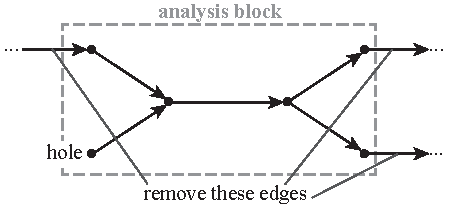
\includegraphics[width=3in]{images/analysis_block_hole}
        \end{center}
        \vspace{-20pt}
    \caption{Example variable node indicating a hole.}
    \label{f:hole}
    \end{figure}

    \item[\bf{Step 2: Collisions}] 
        The second step is to detect collisions and to disconnect precisely the number of connection edges required such that all collisions are resolved without introducting holes. 
        The set of variable nodes at which collisions occur is 
    \begin{equation}
    S_\txt{nodes} = \{v \in V_{M,\txt{var}} \st \txt{deg}^-(v) > \txt{deg}_u^-(v) \},
    \end{equation}
where the degree is now calculated with respect to $F_1$.
    For each collision node we can construct a set containing the edges directed into the node. The set containing all of these sets is constructed as
    \begin{equation}
        S_\txt{edges} = \big \{ \{(x,y) \in E_M\} \ \big| \ y \in S_\txt{nodes} \big \}
    \end{equation}
    Let $J=\{1,2,\ldots,|S_\txt{edges}|\}$ be an indexing set for $S_\txt{edges}$ such that each $S_{\txt{edges},j}$ corresponds to a set in $S_\txt{edges}$ for $j \in J$. 
    An example collision is shown in Fig.~\ref{f:collision} to exemplify the definition of $S_{\txt{edges},j}$. 
    $J$ also indexes $S_\txt{nodes}$ because there is a one--to--one correspondence between the elements in $S_\txt{nodes}$ and the elements in $S_\txt{edges}$ (which are sets). 
    We may then construct sets of edges as
\begin{IEEEeqnarray*}{rCl}
    B_j =  &\big\{& e_k \in S_{\txt{edges},j} \st k \in \{1,2,\ldots,K\} \\
& & \txt{ with } \txt{deg}_u^-(v_j) \leq K \leq \txt{deg}_u^-(v_j) \big \}, \ j \in J,
\end{IEEEeqnarray*}

        which means that each set $B_j$ is constructed from the set $S_{\txt{edges},j}$ by taking only as many edges as are allowed by the upper and lower indegree limits of $v_j$.  
The construction of each $B_j$ corresponds to making a decision about which edges to include and which edges not to include. 
Let the new set of connection edges be denoted
    \begin{equation}
    E_{F_2,\txt{con}} = \{ e \in E_{F_1,\txt{con}} \st e \in B_j \txt{ for some } j \in J\}.
    \end{equation}
The set of all edges is created by removing the connection edges not in $E_{F_2,\txt{con}}$:
    \begin{equation}
    E_{F,2} = E_{F_0} \setminus (E_{M,\txt{con}} \setminus E_{F_2,\txt{con}}),
    \end{equation}
    which gives
    \begin{equation}
    F_2 = (V_{F_0},E_{F_2}).
    \end{equation}
    \begin{figure}[htb!]
        \begin{center}
        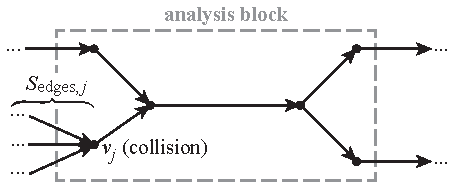
\includegraphics[width=3in]{images/analysis_block_collision}
        \end{center}
        \vspace{-20pt}
    \caption{Example variable node indicating a collision.}
    \label{f:collision}
    \end{figure}

    \item[\bf{Step 3: Finalize}] 
        The third and final step is to prune the graph to exclude any analysis blocks that became unneeded after the collisions were resolved.
        This is accomplished by first creating the reverse graph of $F_2$, $R = (V_R,E_R)$, where
	\begin{equation}
	E_R = \{ (x,y) \st (y,x) \in E_{F_2}\}, \ V_R = V_{F_2}
	\end{equation}
	Next, a new node $b$ is added to $V_R$ and edges directed from this node to each of the expression blocks are added:
    \begin{equation}
        \forall i \in I_E,\forall v \in V_{E_i}, \txt{ if } \txt{deg}^-(v)=0 \txt{ then } (b,v) \in E_R.
    \end{equation}
        The set of nodes that may be reached from $b$ is then constructed as
    \begin{equation}
        U = \{ v \in V_R \st \exists P \txt{ a path from $b$ to $v$}, \ P \subset R \}.
        \end{equation}
	Because $b$ is directed into only the expression blocks, any path from $b$ necessarily provides a path from at least one expression block, which means the node is being used in the problem formulation.

        The list of analysis blocks with at least one node in $U$ is constructed as
        \begin{equation}
        I_F = \{ i \in I_A \st V_{A_i} \cap U \neq \emptyset \}
        \end{equation}
        Any analysis block not in $I_F$ should be removed from the graph because none of its outputs contribute to the problem. Inputs that are not being used are also removed. The set of nodes to remove is then
        \begin{equation}
        N = (V_\txt{in}\setminus U )  \cup \left( \bigcup_{i \notin I_F} V_{A_i} \right),
        \end{equation}
and the new set of nodes is created as
        \begin{equation}
        V_F = V_{F_2} \setminus N.
        \end{equation}
        Edges involving the removed nodes are also deleted as
        \begin{equation}
        E_F = E_{F_2} \setminus \{ (x,y) \st x \in N \txt{ or } y \in N  \}.
        \end{equation}

The fundamental problem graph is then
\begin{equation}
F = (V_F,E_F).
\end{equation}
        If desired, the set of connection edges can be extracted by considering only edges whose endpoints are not in the same analysis block:
\begin{IEEEeqnarray*}{rCl}
E_{F,\txt{con}} = &\{&(x,y) \in E_{F} \st \sim(x \in V_{A_i} \txt{ and } y \in V_{A_i}  \\
& & \txt{for some } i \in I_F)\}.
\end{IEEEeqnarray*}
\end{description}

This algorithm will always provide an FPG if one exists. If an FPG does not exist, the implementation reveals the limiting factors that prevent a valid FPG from being achieved.

\subsection{Suggested Process for Appyling the FPG Algorithm}
\label{ss:process}
Section \ref{ss:obtaining FPG} provided an algorithm for obtaining an FPG from the given MCG. 
The algorithm can be applied as part of a broader process in which the designer changes the problem formulation or the supplied analysis tools to attempt to obtain an FPG. The following steps detail the suggested procedure for obtaining an FPG:
\begin{enumerate}
\item[\bf{(A)}] Begin with a set of inputs, analysis tools, objectives, and constraints.
\item[\bf{(B)}] Build the MCG as described in Sec.~\ref{ss:MCG}.
\item[\bf{(C)}] Set indegree limits for variable nodes representing local inputs as described in Sec.~\ref{s:indegree-outdegree} and Table \ref{t:variable node classification}.
\item[\bf{(D)}] Run the FPG algorithm described in Sec.~\ref{ss:obtaining FPG}. If a valid FPG is unattainable:
		\begin{enumerate}
\item Change the MCG by adding analysis blocks and/or inputs, which means identifying new analysis tools to include in a potential MDAO workflow.
\item Change indegree limits (see Table \ref{t:variable node classification}).
\end{enumerate}
\item[\bf{(E)}] Repeat from step (A) until an FPG is obtained.
\end{enumerate}
This process illustrates how the algorithm for obtaining a valid FPG can be applied. However, the process also serves to illustrate how a designer may revist the MCG after an FPG has already been produced. For example, if a designer desires to change an input to be multi-fidelity, new analysis blocks can be added to the original MCG, the indegree limits can be modified accordingly, and the algorithm can be applied again.
\section{Example Problem}
	\label{s:example problem}
	This section presents an example problem to demonstrate the process of obtaining the FPG and the advantages of doing so. The algorithm from Sec.~\ref{s:building graphs}.\ref{ss:obtaining FPG} was implemented in the NetworkX package of the Python programming language. Any language with the ability to manipulate a graph should be applicable. NetworkX was chosen due to the built--in features, such as cycle detection.

	The example task is the conceptual sizing of a single--aisle subsonic transport using an MDAO framework with objectives for performance and total weight for a required mission. The full set of analysis codes available for use is given in Table \ref{t:analysis codes}.
	\begin{table}[htbp]
	  \centering
	  \caption{Analysis codes for subsonic transport sizing}
		\begin{tabular}{cc}
		\toprule
		analysis code & description \\
		\midrule
		VSP   & parametric geometry \\
		PDCYL & wing and fuselage weight estimation \\
		NPSS  & engine sizing and performance \\
		VORLAX & aerodynamics using the vortex lattice method \\
		PMARC & aerodynamics using a low-order panel method \\
		WATE  & engine weight estimation \\
		FLOPSa & mission performance, \\
		  & engine sizing, and weight estimation \\
		FLOPSb & mission performance only \\
		\bottomrule
		\end{tabular}%
	  \label{t:analysis codes}%
	\end{table}%
	Each of these analysis codes contribute individual disciplinary analysis but they are not mutually exclusive. For example, VORLAX and PMARC are both aerodynamics codes that predict inviscid drag but with different levels of fidelity. The Flight Optimization System (FLOPS) is included twice to represent two different uses. FLOPSa denotes FLOPS being executed for both mission performance and engine analysis, while FLOPSb indicates that FLOPS is executed for only mission performance analysis. This sort of representation is useful for ``supercodes'' that care capable of being used in different ways and with different sets of inputs and outputs.

	In this example, the MCG is formed using a consistant variable naming convention and then connecting every variable with the same name, though this is not the only way to form an MCG. 
	Table \ref{t:ins and outs} presents the full list of variables in the leftmost column and then indicates whether the variable is an input or an output of each analysis code. 
	Some of the variables, such as geometry and performance, represent many different variables which have been bundled together due to there similarity. 
	This bundling is not necessary and does not limit the generality of this example, it is done to simplify the presentation.
	\begin{table}[htb!]
	  \centering
	  \caption{Analysis code input and output description}
		\begin{tabular}{ccccccccc}
		\toprule
		variable & \multicolumn{8}{c}{analysis code} \\
		\midrule
			  & VSP   & PDCYL & NPSS  & VORLAX & PMARC & WATE  & FLOPSa & FLOPSb \\
		geometry & in    & in    &       & in    & in    & in    & in    & in \\
		number of engines &       &       & in    &       &       &       & in    & in \\
		mission &       &       &       &       &       &       & in    & in \\
		fuselage weight &       & out   &       &       &       &       & in    & in \\
		wing weight &       & out   &       &       &       &       & in    & in \\
		engine weight &       &       &       &       &       & out   & out   & in \\
		wetted area & out   &       &       &       &       &       & in    & in \\
		inviscid drag &       &       &       & out   & out   &       &       & in \\
		drag  &       &       & in    &       &       &       & out   & out \\
		engine performance &       &       & out   &       &       & in    & out   & in \\
		performance &       &       &       &       &       &       & out   & out \\
		total weight &       & in    &       &       &       &       & out   & out \\
		\bottomrule
		\end{tabular}
	  \label{t:ins and outs}
	\end{table}

	The MCG $M$ is formed in four steps:
	\begin{enumerate}
	\item An analysis block is created for each analysis code using the information in each column of Table \ref{t:ins and outs}. Each analysis block is formed by creating variable nodes for each input and directing them into a single model node, which is directed into another model node, which is then directed into variable nodes corresponding to each output. 
	A sample analysis block is shown for analysis code FLOPSb in Fig.~\ref{f:FLOPSb analysis block}.
	\begin{figure}[htb!]
	  \begin{center}
		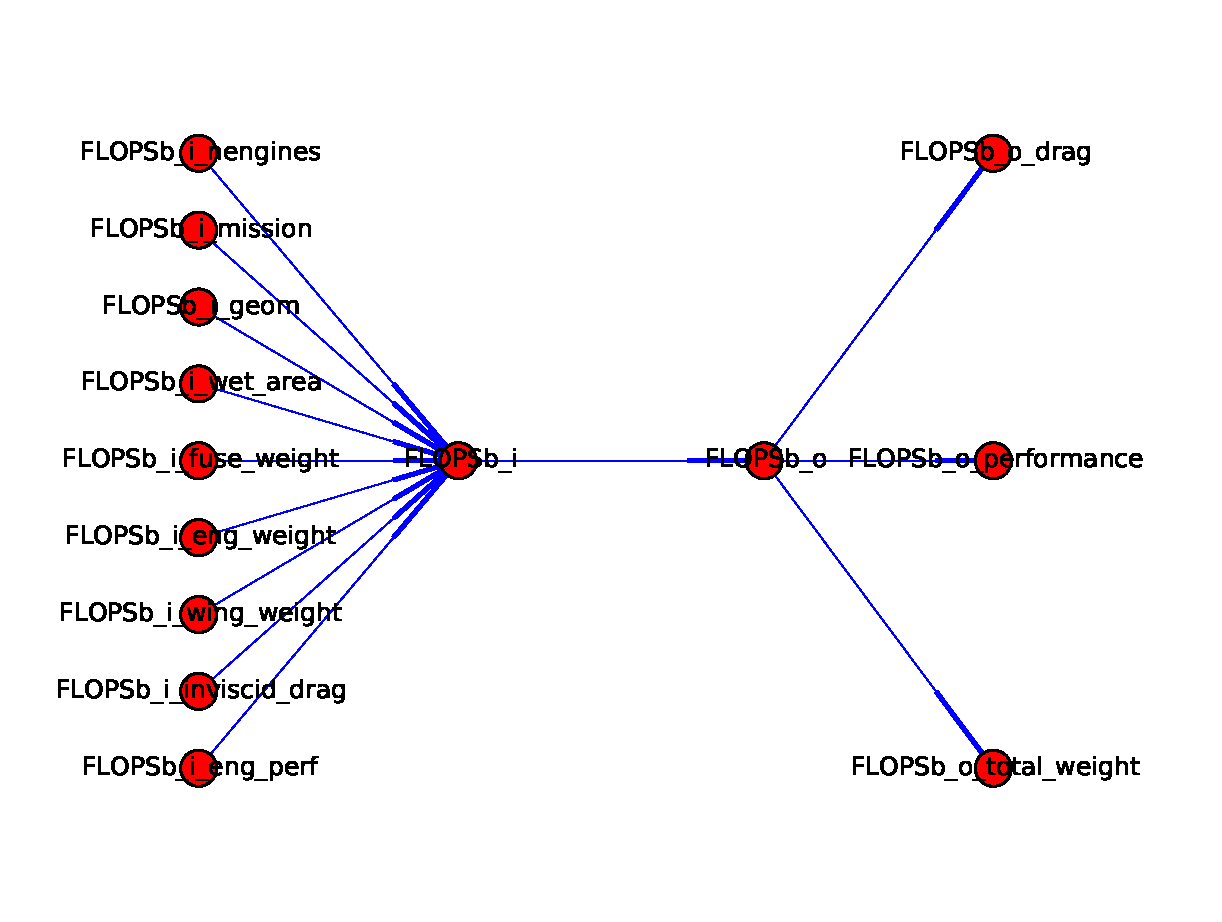
\includegraphics[width=.6\textwidth]{images/FLOPSb_analysis_block}
	  \end{center}
	  \caption{Sample analysis block for analysis code FLOPSb using Table \ref{t:ins and outs}}
	\label{f:FLOPSb analysis block}
	\end{figure}

	\item Variable ((change)) nodes are created to represent the objectives for performance and total weight.

	\item Variable nodes are created to represent the geometry variable and mission variable as global inputs.

	\item Explicit edges are created from each variable node to every other variable node representing variables with the same name. The direction is determined by whether the variable node has an edge directed into or out of a model node (local input or local output).
	\end{enumerate}
	The resulting MCG is shown in Fig.~\ref{f:design vars}. Emerging cycles are shown in yellow and indicate potential cycles that may exist when an FPG is formed.
	\begin{figure}[htb!]
	  \begin{center}
		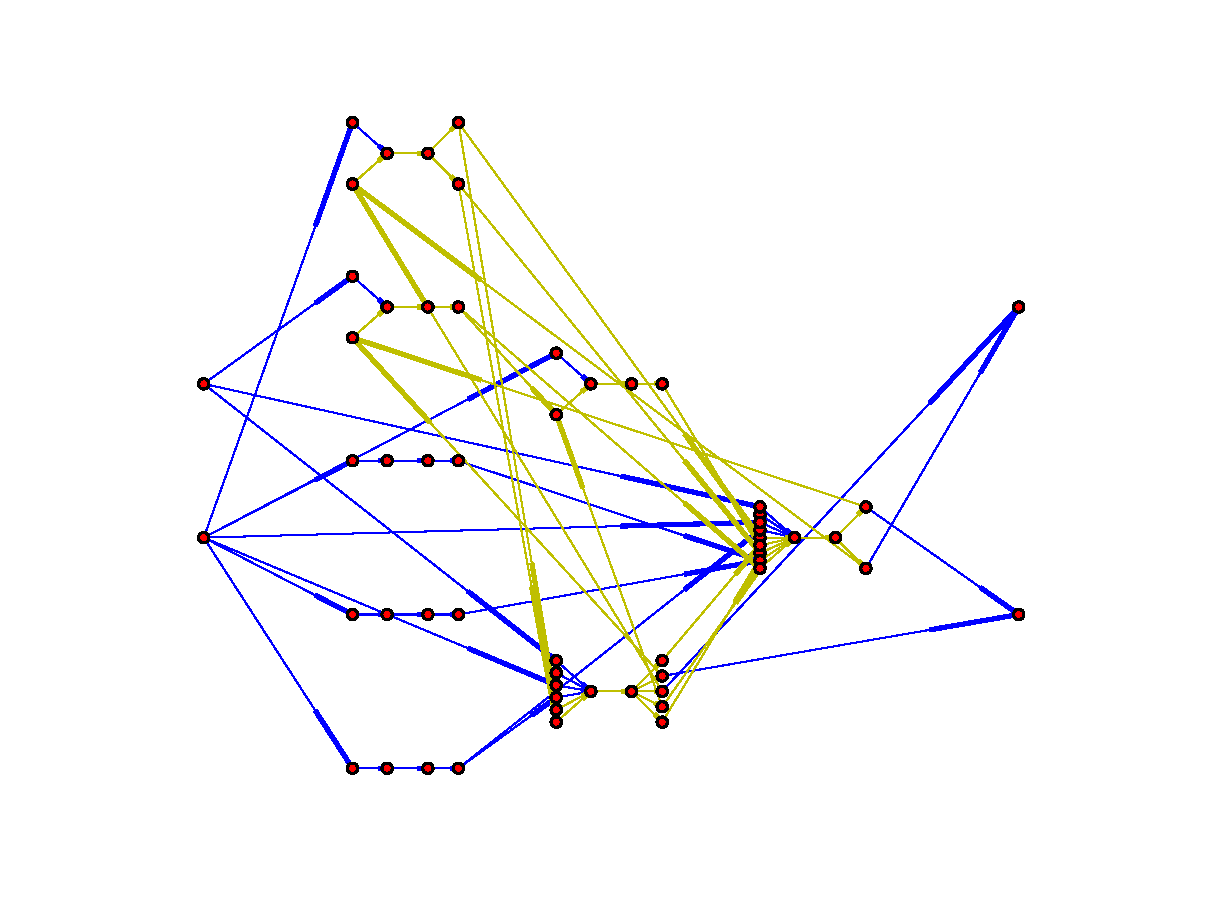
\includegraphics[width=.6\textwidth]{images/MCG}
	  \end{center}
	  \caption{Maximal connectivity graph for the subsonic transport example problem}
	\end{figure}

\subsection{Obtaining an FPG}
	\label{ss:obtaining an FPG}
	The process of obtaining an FPG from the given MCG is expected to be an iterative process in which the user applies the algorithm to determine whether or not an FPG can be obtained, and then modifies the indegree limits or the MCG to obtain a satisfactory FPG. For example, after determining the location of a hole, the user can change the indegree limit to make the node a design variable, or the user could change the MCG by adding a new analysis code such that the hole is resolved.

	As presented in Sec.~\ref{s:building graphs}.\ref{ss:obtaining FPG}, the first step to obtaining an FPG is to detect holes. To start, we set the lower indegree limit for every node to be unity to find any potential holes. In this case, it turns out that the variable nodes representing the number of engines is a hole for NPSS, FLOPSa, and FLOPSb. This implies than an FPG cannot be obtained from the given MCG, as shown in Fig.~\ref{f:MCG nengines}. In this figure, the green nodes indicate analysis blocks with a hole, and the cyan nodes indicate analysis blocks that became unused after the invalid analyses were removed ((connections were removed, color edges too)).
	\begin{figure}[htb!]
	  \begin{center}
		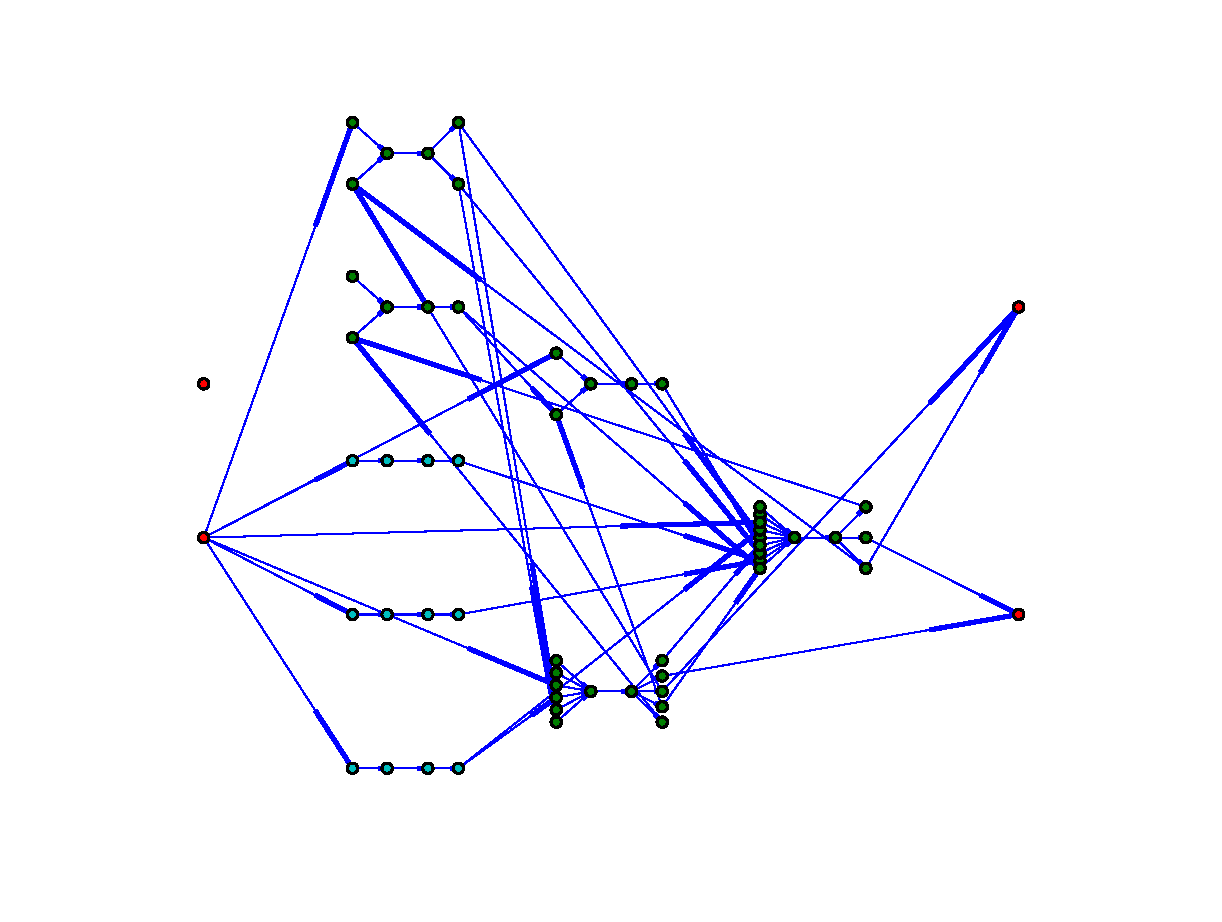
\includegraphics[width=.6\textwidth]{images/MCG_nengines}
	  \end{center}
	  \caption{The MCG with one global variable missing. The resulting holes are shown in green and unused analyses shown in cyan.}
	\label{f:MCG nengines}
	\end{figure}

	Therefore, we may now create another variable node to represent the number of engines as a global input and also create explicit edges to supply this new input. Now this step is repeated with the new MCG and no holes are found.

	While Sec.~\ref{s:building graphs}.\ref{ss:obtaining FPG} indicated the process for obtaining an FPG, it did not specify how to decide which edges to keep when resolving a collision, that freedom is left to the specific implementation. The benefit of this approach is that standard graph theory algorithms can be used to make these decisions. The first example of this is to obtain an FPG with the fewest possible number of cycles, which are found using the implementation of Johnson's algorithm \cite{Johnson1975} in the Python package NetworkX. The FPG with the fewest cycles is shown in Fig.~\ref{f:FPG fewest cycles}, which indicates one cycle shown in yellow. A similar alternative would be to minimize the number of analysis blocks involved in cycles, counting multiplicity.
	\begin{figure}[htb!]
	  \begin{center}
		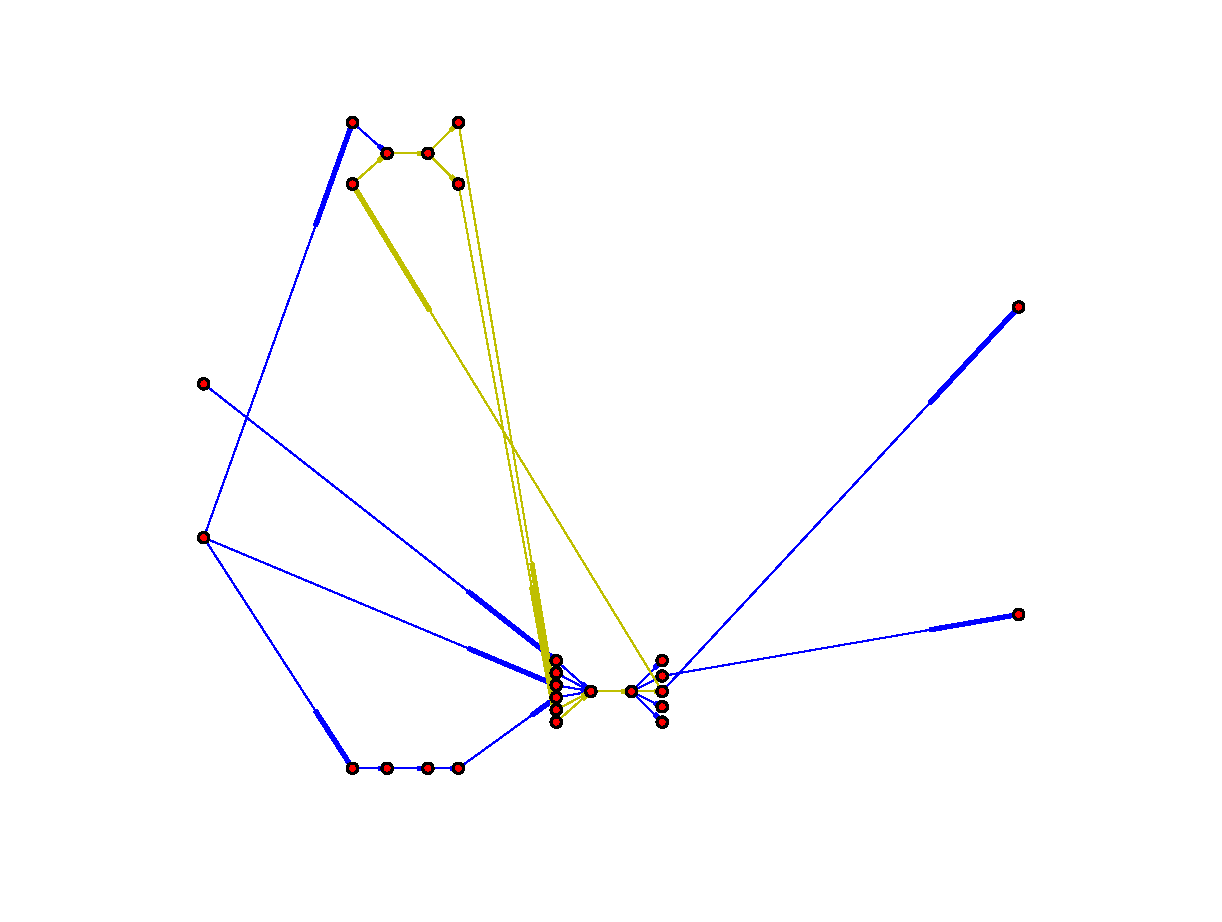
\includegraphics[width=.6\textwidth]{images/FPG_fewest_cycles}
	  \end{center}
	  \caption{FPG with the fewest number of cycles.}
	\label{f:FPG fewest cycles}
	\end{figure}

	Alternatively, it may be desirable to resolving collisions by including the higher fidelity codes, such as NPSS in this case.
	One method to ensure that the edges directed from certain analysis blocks are the ones chosen to resolve the conflicts is to use a ranking system. For this case, consider the rankings for each analysis code given in Table \ref{t:rankings}.
	\begin{table}[htbp]
	  \centering
	  \caption{Example ranking of importance}
		\begin{tabular}{cc}
		\toprule
		analysis code & rank \\
		\midrule
		VSP   & 5 \\
		PDCYL & 5 \\
		NPSS  & 4 \\
		PMARC & 4 \\
		FLOPSb & 4 \\
		VORLAX & 3 \\
		WATE  & 3 \\
		FLOPSa & 2 \\
		\bottomrule
		\end{tabular}%
	  \label{t:rankings}%
	\end{table}% 
	Step two in Sec.~\ref{s:building graphs}.\ref{ss:obtaining FPG} (the resolution of collisions) is now conducted by selecting the edges directed from the analysis blocks with the highest rank for each collision. The resulting FPG is shown in Fig.~\ref{f:FPG highest rank}, and this graph has four cycles, which are enumerated in Table \ref{t:cycles}.
	\begin{figure}[htb!]
	  \begin{center}
		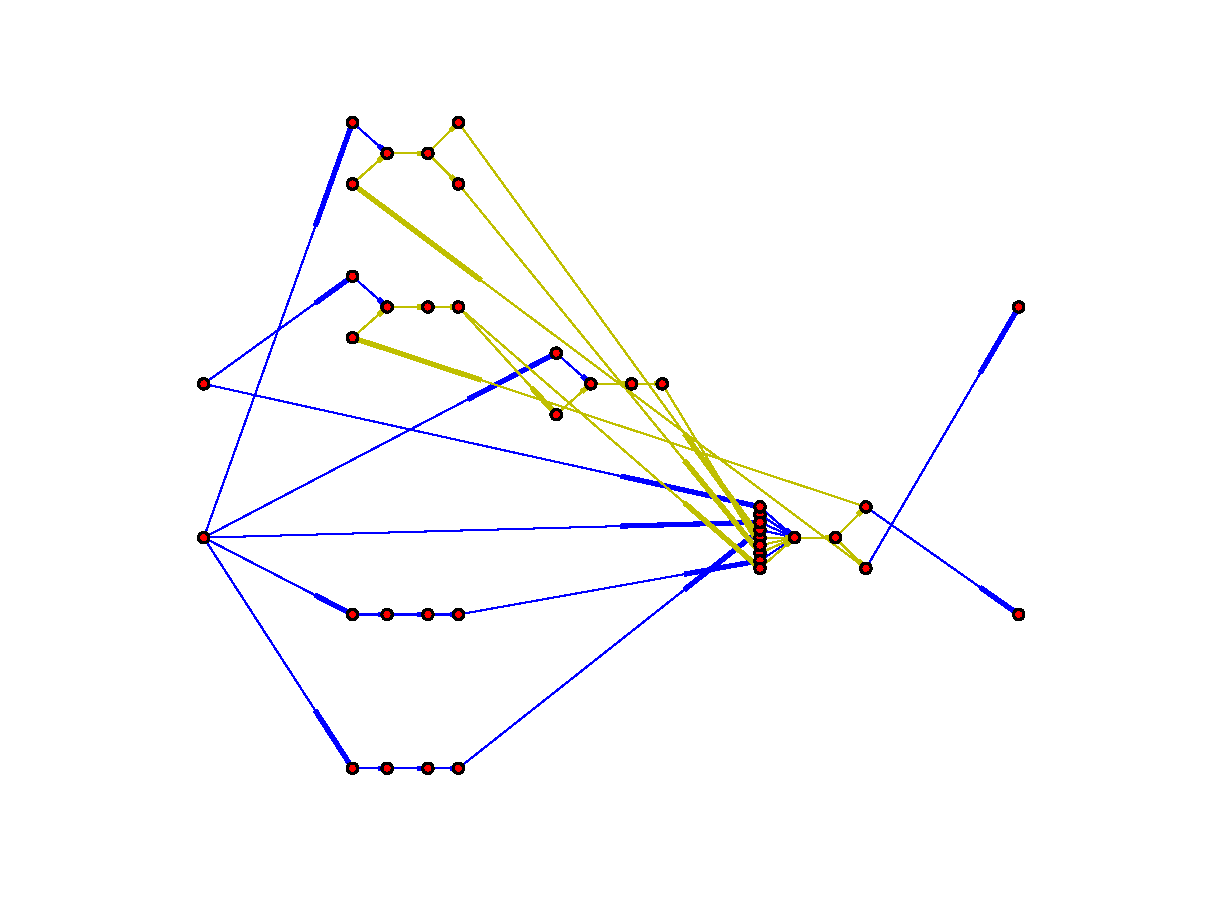
\includegraphics[width=.6\textwidth]{images/FPG_highest_rank}
	  \end{center}
	  \caption{FPG obtained using the ranking system.}
	\label{f:FPG highest rank}
	\end{figure}
	\begin{table}[htbp]
	  \centering
	  \caption{Cycles for the FPG obtained using ranking}
		\begin{tabular}{ccccccc}
		\toprule
		output/input & analysis code & output/input & analysis code & output/input & analysis code & output/input \\
		\midrule
		engine weight & FLOPSb & drag  & NPSS  & engine performance & WATE  & engine weight \\
		engine performance & FLOPSb & drag  & NPSS  & engine performance &       &  \\
		fuselage weight & FLOPSb & total weight & PDCYL & fuselage weight &       &  \\
		wing weight & FLOBSb & total weight & PDCYL & wing weight &       &  \\
		\bottomrule
		\end{tabular}%
	  \label{t:cycles}
	\end{table}%

	Finally, now consider the case where it is desired to have the inviscid drag input into FLOPSb be a multi--fidelity input, meaning that it is sought to use multiple analysis codes to calculate the same variable. This is done simply by setting the upper indegree limit for this node as two and then repreating the (automated) process. In this case, both VORLAX and PMARC are retained, resulting in an FPG that omits only FLOPSa.


%\begin{figure}[htb!]
%  \begin{center}
%    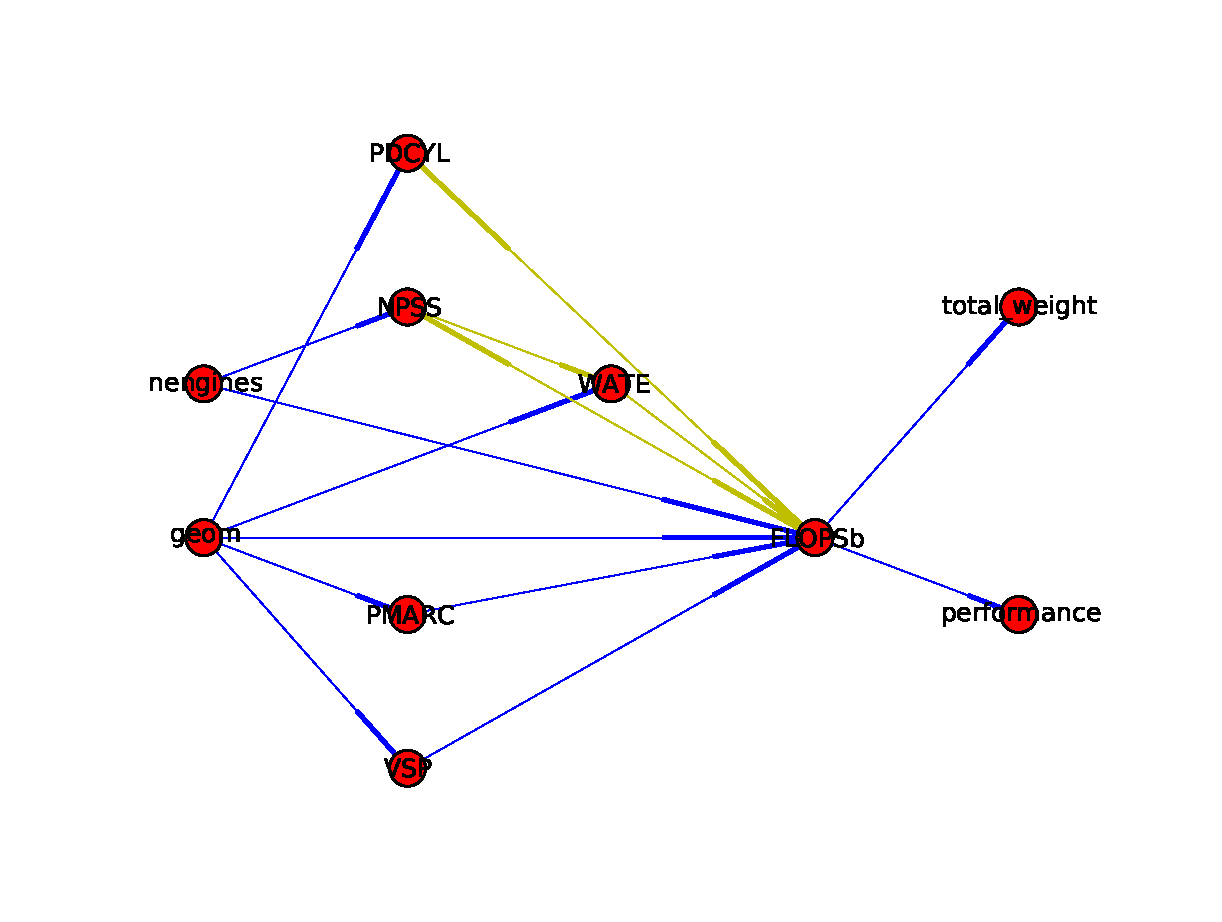
\includegraphics[width=.6\textwidth]{images/FPG_highest_rank_simplified}
%  \end{center}
%  \caption{Simple notional problem with two potential design variables \label{f:design vars}}
%\end{figure}






%\begin{table}[h!]
% \begin{center}
%  \caption{Example problem analysis codes}
%  \label{t:analysis codes}
%  \begin{tabular}{ccc} \hline 
%Analysis code & input variables & output variables \\ \hline
%VSP & geometry & wetted area \\
%PDCYL & geometry & fuselage weight \\
%	& total weight & wing weight \\
%NPSS & number of engines & engine performance \\
%	& drag &	\\
%VORLAX & geometry & inviscid drag \\
%PMARC & geometry & inviscid drag \\
%WATE & geometry & engine weight \\
%	& engine performance &	\\ 
%FLOPSa & number of engines & engine weight \\
%	& mission & performance \\
%	& geometry & total weight \\
%	& wetted area & engine performance \\
%	& fuselage weight & drag \\
%FLOPSb & number of engines & drag \\
%	& mission & performance \\
%	& geometry & total weight \\
%	& wetted area & 	 \\
%	& engine weight & 	\\
%	& wing weight & 	\\
%	& inviscid drag & 	\\
%	& engine performance & 	\\ \hline
%  \end{tabular}
% \end{center}
% \vspace{-15pt}
%\end{table}


\section{Applications}

\section{Conclusions}

\bibliography{library}
\end{document}
